\chapter*{General Introduction}
\addcontentsline{toc}{chapter}{General Introduction}
\begin{figure}[H]
\vspace{.3in}
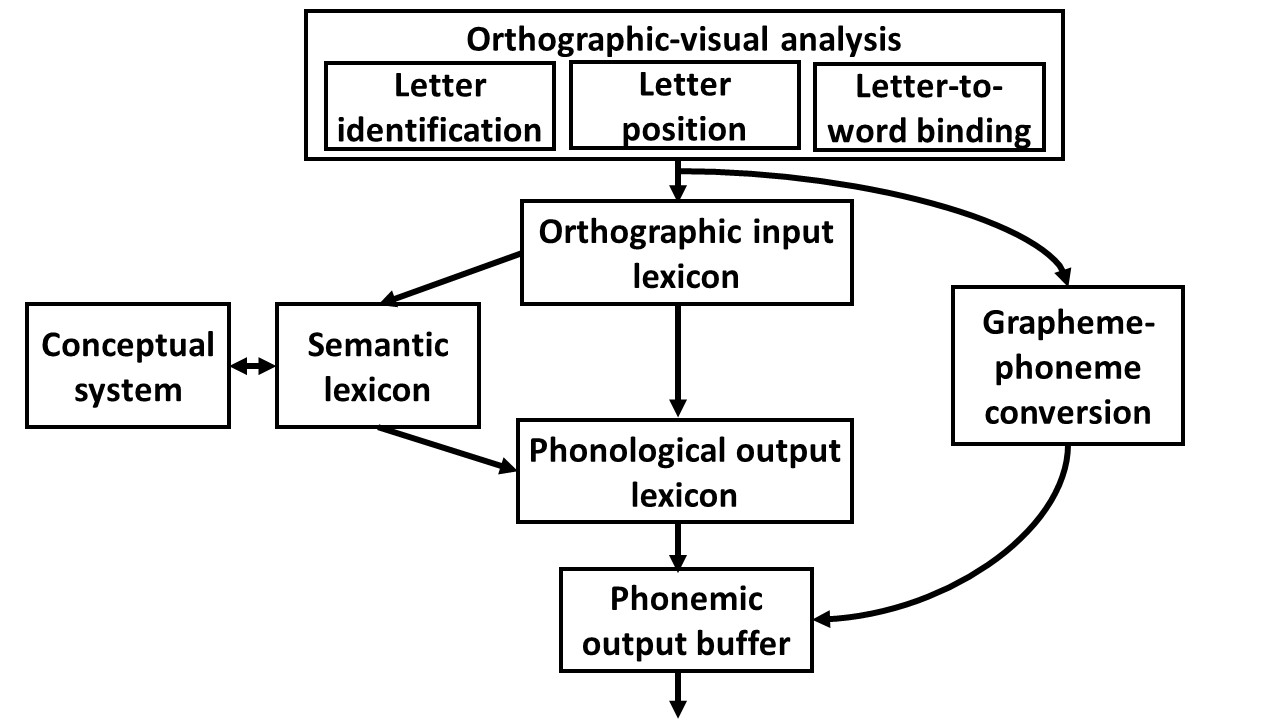
\includegraphics[width=\linewidth]{Figures/Ch1/DualRoute}
\caption{The dual-route model \citep{friedmann2016types})}
\end{figure}

Reading is a complex and unique skill of the human brain. Reading aloud requires the brain to perform multiple low and high level processes, such as graphical pattern recognition, composition of letters into words, grapheme-to-phoneme conversion, phoneme production and, regularly, ascription of meaning – all almost in parallel and in strikingly short time and accuracy. Reading is thus a fertile ground for studying many processes that take place in the brain. Much can be learned about our visual, auditory, and motor system, and their interactions, from its investigation.

\citet{mn73} were the first to distinguish different subtypes of dyslexia, and the first to propose a cognitive model of reading which accounts for these different subtypes. The model proposed was a Dual-Route model, in which reading takes place in two routes, which are activated in parallel. One route, the lexical route, serves for reading already known words, and is characterized by fast retrieval of words from long-term memory lexicons. The second route, the sub-lexical route, serves for reading new, non-familiar words, and is characterized by step-by-step conversion of graphemes to phonemes. In this model, each subtype of dyslexia, associated with specific error types, was to be explained by a malfunction of a specific locus in the model. With time, the discovery of new characteristic error types, that is, new subtypes of dyslexia, led to the modification and refining of the reading model. Figure 1 describes the most accepted version of the Dual-Route Model.

According to this model, the first stage of the reading process consists of an Orthographic-Visual analysis (hereafter, OV analysis). In this stage three processes take place: (1) the encoding of the identity of the letters (2) the encoding of the relative positions of letters within the word, and (3) letter-to-word binding by allocating attention to a single word. A malfunction in any of these processes will correspond to a specific subtype of dyslexia. For example, a malfunction in the relative position allocation will cause a Letter Position Dyslexia (LPD) \citep{friedmann2001letter, friedmann2005letter}, a characteristic error of which would be reading e.g. ‘broad’ as ‘board’. A malfunction of the binding of a letter to the word in which it appears is called Attentional Dyslexia, a characteristic error of which would be reading ‘High Way’ as ‘High Hay’ (e.g., \citealp{sw77}). As seen in Figure 1, the output from the OV analysis stage, containing the information about the identities and relative positions of the letters, flows in parallel into the two routes – the lexical route (‘OV Analysis - ‘Orthographic Input Lexicon’ – ‘Phonological Output Lexicon’ – ‘Phonemic Output Buffer’) and the sub-lexical route (‘OV Analysis - ‘G2P conversion’ – ‘Phonemic Output Buffer’). With regards to the sub-lexical route, recent evidence has rendered it a point of interest for research. 

A general malfunction of the sub-lexical route, identified several decades ago, is called Phonological Dyslexia (for review, see \citealp{c96}). Individuals with this type of dyslexia can read words with which they are already familiar (words that exist in their orthographic input lexicon – Figure 1), but they make errors in reading non-familiar words. Recently, more specific subtypes of dyslexia of the sub-lexical route were reported. \citet{Gvion2010} reported a new intriguing subtype of dyslexia. They reported a person with selective conversion impairment reading ‘goat’ as ‘coat’ and ‘pear’ as ‘bear’ thus having voicing substitution errors. They therefore coined this dyslexia as ‘Dyslegzia’. Another case \citet{Gvion2012} reported suggested that voicing is not the only feature that can be selectively impaired in reading. They reported a case in which the nasality feature was affected (alongside the voicing feature). Last, \citet{kf11} reported a new sub-lexical route dyslexia, in which only vowels are affected and not consonants – Vowel Letter Dyslexia. They reported 25 cases of individuals making errors of migrations, substitutions, omissions, or additions of a vowel letter, and showed, as for all the above subtypes of dyslexia, converging evidence that the impairment was located in the sub-lexical route and not in a different locus of the Dual-Route reading model.

Given this seemingly complex structure of the reading process and different types of reading errors, we propose to model these phenomena with computational tools. chapter 1 explores the generation process of reading-errors with probabilistic graphical models. It addresses a long-lasting debate in neurolinguistics, regarding the heterogeneity of dyslexia - whether dyslexia should be discerned into subtypes, or rather it has one single cause \citep{s98, s00}. It proposes a new path to the problem, by adopting a data-driven approach - letting the data "to speak for itself" - and makes use of probability language to capture the complex generation process of reading errors. In this study, we construct learning algorithms that can discover possible hidden patterns in the data, thus illuminating on the issue in question. In addition, the study develops an automatic diagnostic tool of subtypes of dyslexia, based on error types, which lays the groundwork for easily accessible, cheap and fast screening tests. 

The next two chapters study the basic elements of spoken words, that is, phonemes, which underlie many sub-processes during reading. Their primary motivation is to explain the existence of phoneme-related subtypes of dyslexia, such as dyslegzia, or vowel-letter dyslexia, but the absence of other possible dyslexia subtypes - there are no known subtypes of dyslexia that specifically affect other phonological features except for the above-mentioned ones (voicing, nasality, vowels and evidences for substitutions among strident phonemes). For example, there is no evidence for a deficit that generates phoneme substitutions related to the [labial] feature. It is therefore enigmatic why some phoneme-related errors are more common in reading than others.

The answer to this question may lie in the similarity relations among phonemes. Phoneme-related reading errors may follow phoneme similarity. Various studies have suggested means to measure phoneme similarity \citep{NicelyMiller1955} or compute it from subphonemic features (e.g., \citealp{Pierrehumbert1993}). However, given a theory of phonological features, it is unclear what is the contribution of each feature to the overall similarity. A difference with respect to some phonological features may make a pair of phonemes more perceptually distinguishable compared to differences in other features, thus less similar. For example, a difference with respect to nasality ([+nasal] vs. [-nasal]) as in /n/-/d/, may render the two more distinguishable compared to a difference with respect to, e.g., [labial] as in /n/-/m/. To answer the question about the prevalence of phoneme-related subtypes of dyslexia, it seems crucial to quantify the contribution of various phonological features to the overall similarity. Differences among features with respect to their perceptual saliency, may explain differences in prevalence of phoneme-related subtypes of dyslexia. chapter 2 proceeds in this direction and proposes a new methodological approach to the question of phoneme similarity. The framework is similar in spirit to that of chapter 1, adopting a data-driven approach, and differs from previous studies in phonology, which manually devised similarity functions (e.g., \citealp{Frisch1997}). We test the approach on several feature theories and phoneme-similarity datasets, including a new dataset that we collected for Hebrew.  

Chapter 3 complements the inquiry into phoneme similarity from a neuroscientific point of view. It tests the dominance of various phonological features in neural representations of phonemes, as revealed from neural activity in auditory regions. We collected spiking activity from single neurons in high-level auditory regions in the superior temporal gyrus, while aurally presenting consonant-vowel and vowel stimuli to neurosurgical patients implemented with deep electrodes. We then characterize the functional organization of phonemes from spiking activity, and quantify the dominance of various phonological features in the neural representations. Finally, we compare the neural representations and the perceptual similarities among phonemes from chapter 2. Taken together, the studies provide a characterization of both neural and cognitive similarity structures among phonemes.